\documentclass{article}
\usepackage[margin=1.2in]{geometry}
\usepackage{graphicx}
\usepackage{caption}
\usepackage{subcaption}

\begin{document}

GWAS analysis report

\section*{SNP data preparation}
The original SNP data is stored in a single VCF file and was generated according to the following metrics:
\begin{itemize}
	\item SNPs with minor allele frequency less than 5\% were filtered out and
	\item SNPs with maximum missing frequency higher than 10\% were removed.
\end{itemize}
The filtered VCF file from KnowPulse needed further conversion as the chromosome information was missing. Thus, contigs/scaffolds needed to be mapped to genome after the file was generated. However, there were still certain number of contigs/scaffolds unmapped after the conversion. The total number of SNPs is 20811, while the numbers of contigs and scaffolds are 2418 and 694, respectively. Notably, all the names of contigs are preceded with chromosome numbers. While it was neither safe to directly replace such contigs with chromosome numbers nor was it wise to ignore all of them, such contigs were mapped to faked chromosomes for future analysis. For instance, if a SNP comes from a contig whose chromosome number is 1, we mapped the contig to 8, i.e., 1 + 7, given that there are 7 chromosomes in lentil genome. The remaining unmapped scaffolds were mapped to Chromosome 15.

On top of that, PLINK was applied to transform the data format into bed/bim/fam/ped/map, which could be accepted by the mainstream GWAS software packages, \emph{e.g.}, PLINK, FaST-LMM, TASSEL, \emph{etc}. 

Since samples coming from a same family yet growing in different regions have only one copy of SNPs, duplication of SNPs for samples is needed. By doing so, we assumed that the genetic materials among samples within one family were equivalent (needs citation here). 

\section*{Covariant data preparation}
Other than the two different types of environmental data, \emph{i.e.}, precipitation and day length, seed weight was also taken into account. To comply with file format required by GWAS packages, \emph{i.e.}, PLINK and FaST-LMM, PLINK was employed to aggregate the genotype, covariate and phenotype data. 

\section*{GWAS analysis via PLINK}
PLINK is the gold standard to do GWAS analysis as it is fast and is equipped with multiple functionalities (cite Alarcon \emph{et al.}), \emph{e.g.}, data management, summary statistics, population stratification and association analysis (cite Purcell \emph{et al.}). In our case, other than the data management functionality that was applied to transform the VCF into other file formats,  summary statistics was applied to describe the genome coverage, whereas the association analysis tool was employed to examine how genes interact with phenotypes, \emph{i.e.}, days to emergence and growing degree days. 

Since the purpose of GWAS is to tell which SNPs are playing significant roles in our observed traits, association analyses of both quantitative and binary traits were conducted in this study. The distributions of the two phenotypic datasets are shown in Fig~\ref{fig:hist}.

\begin{figure}[!htb]
\centering
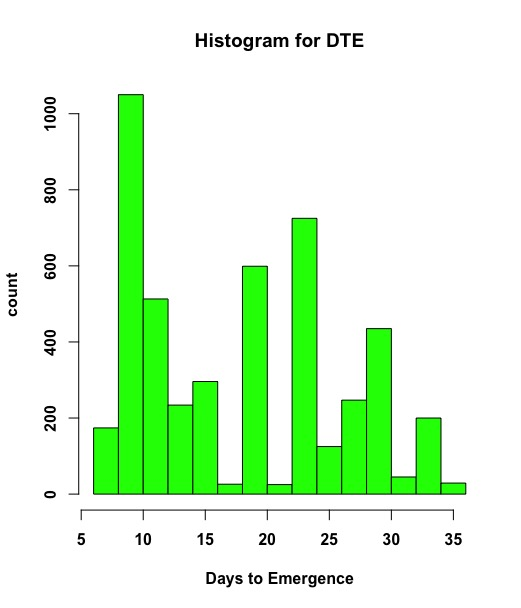
\includegraphics[scale=.35]{hist_dte.jpeg}
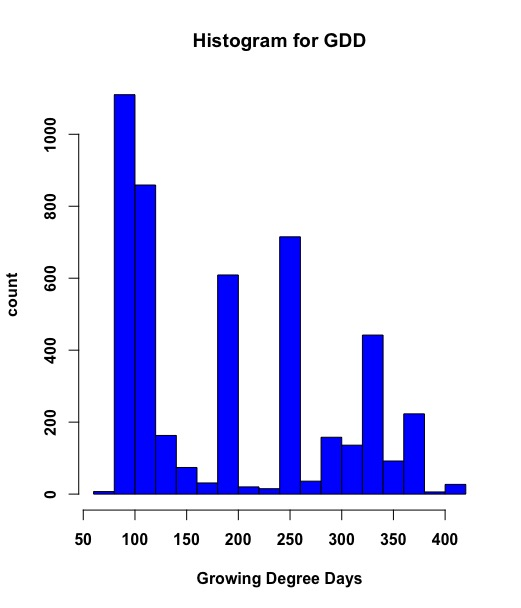
\includegraphics[scale=.35]{hist_gdd.jpeg}
\caption{Histograms of DTE and GDD datasets}
\label{fig:hist}
\end{figure}

The medians of DTE and GDD are 19 and 191.4025, respectively. To do case-control studies over the two traits, samples with DTE less than 19 were grouped into the affected and otherwise the unaffected, whereas samples with GDD less than 191.4025 were grouped into the affected and otherwise the unaffected. The results are shown in Fig~\ref{fig:plink_res}.

\begin{figure}[!htb]
\centering

\begin{subfigure}{\textwidth}
\centering
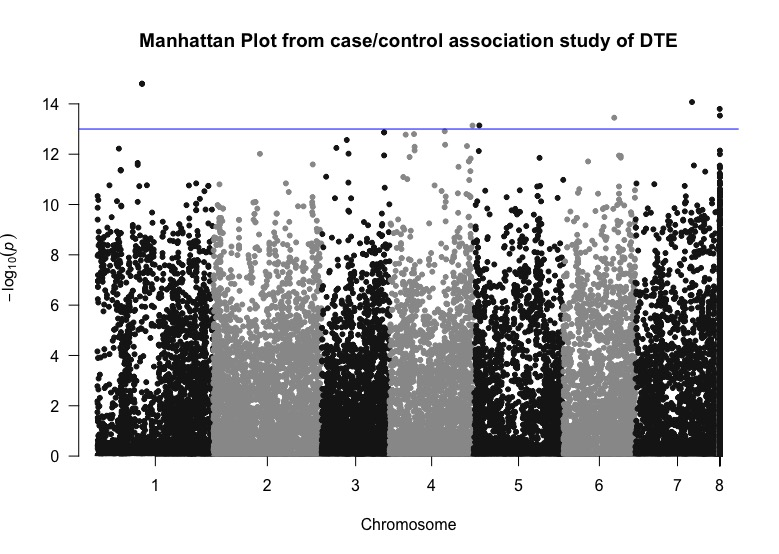
\includegraphics[scale=.25]{mplot_cc_dte.jpeg}
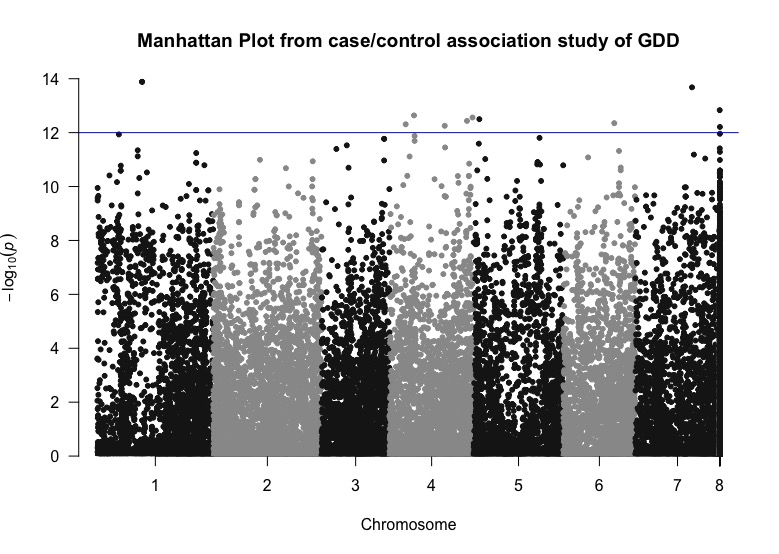
\includegraphics[scale=.25]{mplot_cc_gdd.jpeg}
\caption{Manhattan Plots of days to emergence and growing degree days case-control association studies from PLINK}
\label{fig:plink_sub1}
\end{subfigure}

\begin{subfigure}{\textwidth}
\centering
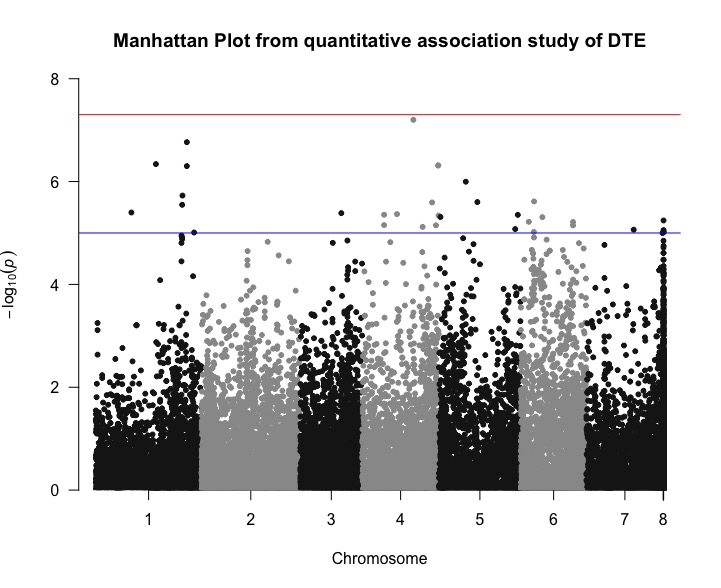
\includegraphics[scale=.25]{mplot_qassoc_dte.jpeg}
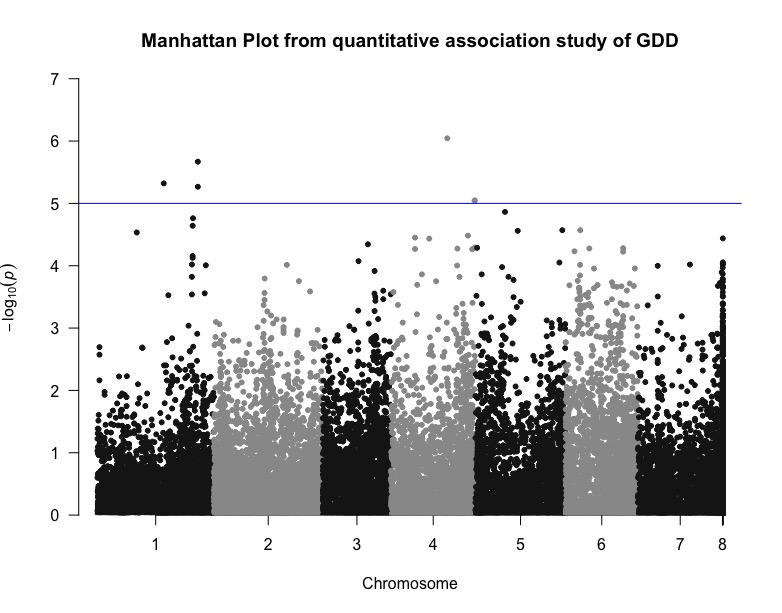
\includegraphics[scale=.25]{mplot_qassoc_gdd.jpeg}
\caption{Manhattan Plots of days to emergence and growing degree days quantitative association studies from PLINK}
\label{fig:plink_sub2}
\end{subfigure}

\caption{Manhattan Plots of association studies from PLINK}
\label{fig:plink_res}
\end{figure}

Table~\ref{table:qassoc_dte} gives the top 6 significant SNP information from PLINK quantitative association study on days to emergence.

\begin{table}[!h]
\centering
\begin{tabular}{|c|c|c|c|c|c|}
\hline
Chromosome & Physical Position & Regression Coefficient & Standard Error & Regression $r^2$ & p-value\textsuperscript{*} \\ [.5ex]
\hline
4 & 163844531 & 07983 & 0.1473 & 0.006817 & 6.290e-8 \\
\hline
1 & 291984120 & 0.9569 & 0.1827 & 0.006173 & 1.711e-07 \\
\hline
1 & 192789217 & 0.9287 & 0.1839 & 0.005688 & 4.571e-07 \\
\hline
4 & 243535564 & 0.6334 & 0.1257 & 0.006004 & 4.860e-07 \\
\hline
4 & 243535565 & 0.6334 & 0.1257 & 0.006004 & 4.860e-07 \\
\hline
1 & 291941752 & 0.8953 & 0.1779 & 0.005745 & 5.002e-07 \\
\hline
\end{tabular}
\flushleft{\textsuperscript{*} Wald Test asymptotic p-value}
\caption{Top SNPs from PLINK quantitative association study on days to emergence}
\label{table:qassoc_dte}
\end{table}

Table~\ref{table:qassoc_gdd} gives the top 6 significant SNP information from PLINK quantitative association study on growing degree days.

\begin{table}[!h]
\centering
\begin{tabular}{|c|c|c|c|c|c|}
\hline
Chromosome & Physical Position & Regression Coefficient & Standard Error & Regression $r^2$ & p-value\textsuperscript{*} \\ [.5ex]
\hline
4 & 163844531 & 8.597 & 1.748 & 0.005621 & 9.042e-07 \\
\hline
1 & 291984120 & 10.300 & 2.170 & 0.005075 & 2.143e-06 \\
\hline
1 & 192789217 & 10.000 & 2.183 & 0.004681 & 4.775e-06 \\
\hline
1 & 291941752 & 9.622 & 2.113 & 0.004707 & 5.409e-06 \\
\hline
4 & 243535564 & 6.637 & 1.493 & 0.004677 & 9.001e-06 \\
\hline
4 & 243535565 & 6.637 & 1.493 & 0.004677 & 9.001e-06 \\
\hline
\end{tabular}
\flushleft{\textsuperscript{*} Wald Test asymptotic p-value}
\caption{Top SNPs from PLINK quantitative association study on growing degree days}
\label{table:qassoc_gdd}
\end{table}

Table~\ref{table:cc_dte} gives the top 6 significant SNP information from PLINK case-control association study on days to emergence.

\begin{table}[!h]
\centering
\begin{tabular}{|c|c|c|c|c|c|c|c|}
\hline
Chromosome & Physical Position & A1\textsuperscript{1} & F\_A \textsuperscript{2} & F\_U\textsuperscript{3} & A2\textsuperscript{4} & ${\chi}^2$ & p-value \\ [.5ex]
\hline
1 & 130505078 & T & 0.4709 & 0.3852 & C & 63.52 & 1.585e-15 \\
\hline
1 & 130505103 & C & 0.4709 & 0.3852 & T & 63.52 & 1.585e-15 \\
\hline
1 & 130505132 & T& 0.4709 & 0.3852 & C & 63.52 & 1.585e-15 \\
\hline
7 & 165628331 & C & 0.3657 & 0.2869 & T & 60.22 & 8.464e-15 \\
\hline
6 & 148586244 & T & 0.3954 & 0.3185 & G & 57.41 & 3.547e-14 \\
\hline
5 & 16655279 & G & 0.4747 & 0.3937 & A & 56.01 & 7.228e-14 \\
\hline
\end{tabular}
\flushleft{
\textsuperscript{1} Minor allele code \\
\textsuperscript{2} Case allele frequency \\
\textsuperscript{3} Control allele frequency \\
\textsuperscript{4} Major allele code
}
\caption{Top SNPs from PLINK case-control study on days to emergence}
\label{table:cc_dte}
\end{table}

Table~\ref{table:cc_gdd} gives the top 6 significant SNP information from PLINK case-control association study on growing degree days.

\begin{table}[!h]
\centering
\begin{tabular}{|c|c|c|c|c|c|c|c|}
\hline
Chromosome & Physical Position & A1\textsuperscript{1} & F\_A \textsuperscript{2} & F\_U\textsuperscript{3} & A2\textsuperscript{4} & ${\chi}^2$ & p-value \\ [.5ex]
\hline
1 & 130505078 & T & 0.4702 & 0.3873 & C & 59.38 & 1.299e-14 \\
\hline
1 & 130505103 & C & 0.4702 & 0.3873 & T & 59.38 & 1.299e-14 \\
\hline
1 & 130505132 & T & 0.4702 & 0.3873 & C & 59.38 & 1.299e-14 \\
\hline
7 & 165628331 & C & 0.3657&  0.2881 & T & 58.45 & 2.081e-14 \\
\hline
4 &  71465726 & T & 0.4738 & 0.3955 & G & 53.74 & 2.293e-13 \\
\hline
4 & 242435083 & G & 0.5103 & 0.4320 & T & 53.38 & 2.742e-13 \\
\hline
\end{tabular}
\flushleft{
\textsuperscript{1} Minor allele code \\
\textsuperscript{2} Case allele frequency \\
\textsuperscript{3} Control allele frequency \\
\textsuperscript{4} Major allele code
}
\caption{Top SNPs from PLINK case-control study on growing degree days}
\label{table:cc_gdd}
\end{table}

To examine how the observed p-values follow an expected pattern, quantile-quantile plots are shown in Fig~\ref{fig:plink_qqplot}.

\begin{figure}[!htb]
\centering

\begin{subfigure}{\textwidth}
\centering
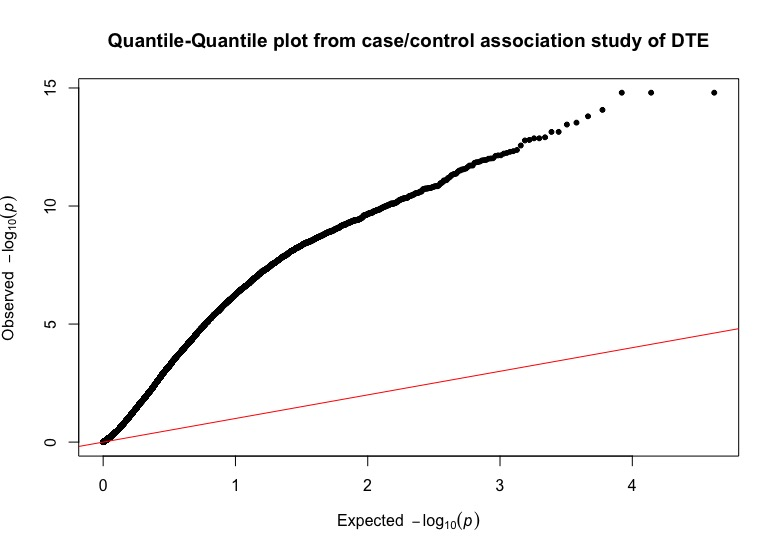
\includegraphics[scale=.25]{qqplot_cc_dte.jpeg}
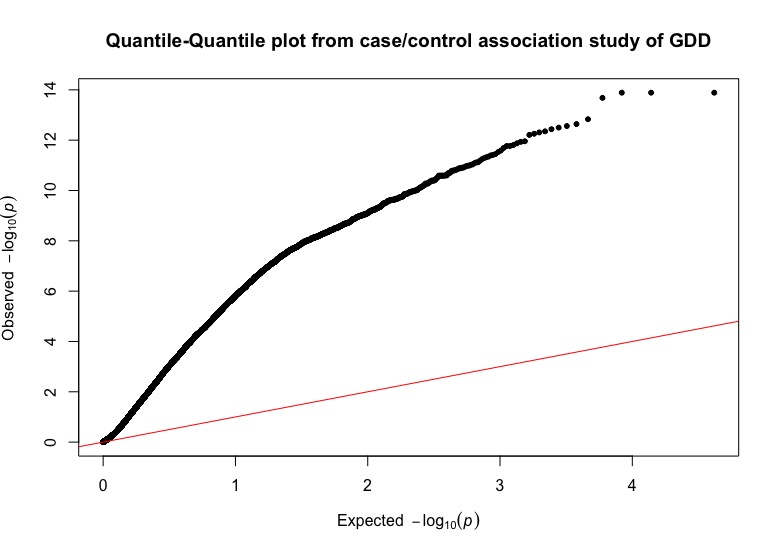
\includegraphics[scale=.25]{qqplot_cc_gdd.jpeg}
\caption{Quantile-quantile plots of DTE and GDD case-control studies from PLINK}
\label{fig:plink_qqplot_sub1}
\end{subfigure}

\begin{subfigure}{\textwidth}
\centering
\includegraphics[scale=.25]{qqplot_qassoc_dte.jpeg}
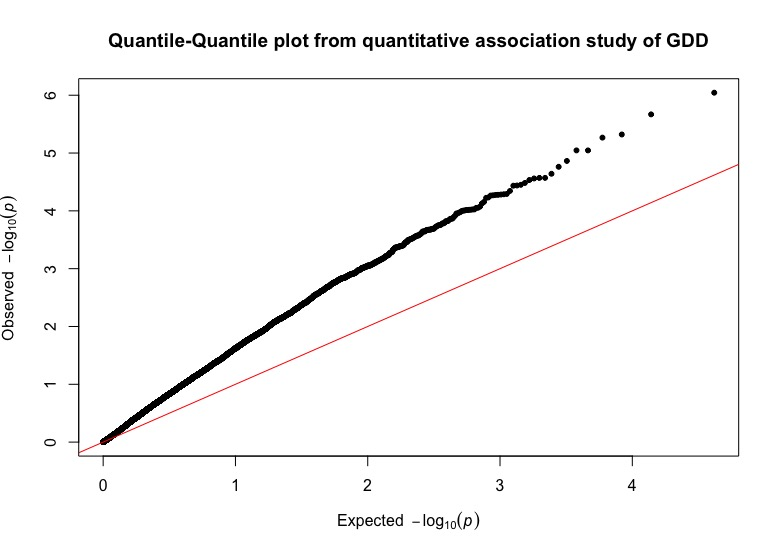
\includegraphics[scale=.25]{qqplot_qassoc_gdd.jpeg}
\caption{Quantile-quantile plots of DTE and GDD quantitative association studies from PLINK}
\label{fig:plink_qqplot_sub2}
\end{subfigure}

\caption{Quantile-quantile plots of association studies from PLINK}
\label{fig:plink_qqplot}
\end{figure}

Although PLINK returned with significant SNPs, as shown in Fig~\ref{fig:plink_sub1} and Fig~\ref{fig:plink_sub2}, the observed p-values tend to be diverged from the expected pattern, as shown in Fig~\ref{fig:plink_qqplot_sub1} and Fig~\ref{fig:plink_qqplot_sub2}. Hence, further investigation on the SNPs needs to be done to determine whether or not they are truly significant in lentil DTE and GDD.

\bigskip

\section*{GWAS analysis via Python FaST-LMM}
The Python FaST-LMM package does GWAS based on a different model (add more details of the FaST-LMM and cite the FaST-LMM paper). Currently, FaST-LMM has gained popularity in lentil GWAS analysis due to the small genome size of lentil. However, unlike PLINK, the Python FaST-LMM package does not output interaction results between genes and environmental factors (cite Alarcon \emph{et al.}). The Manhattan Plot of SNPs with p-values is shown in Fig~\ref{fig:fastlmm_res}

\begin{figure}[!htb]
 \centering
 \begin{subfigure}[normla]{\textwidth}
  \centering
  	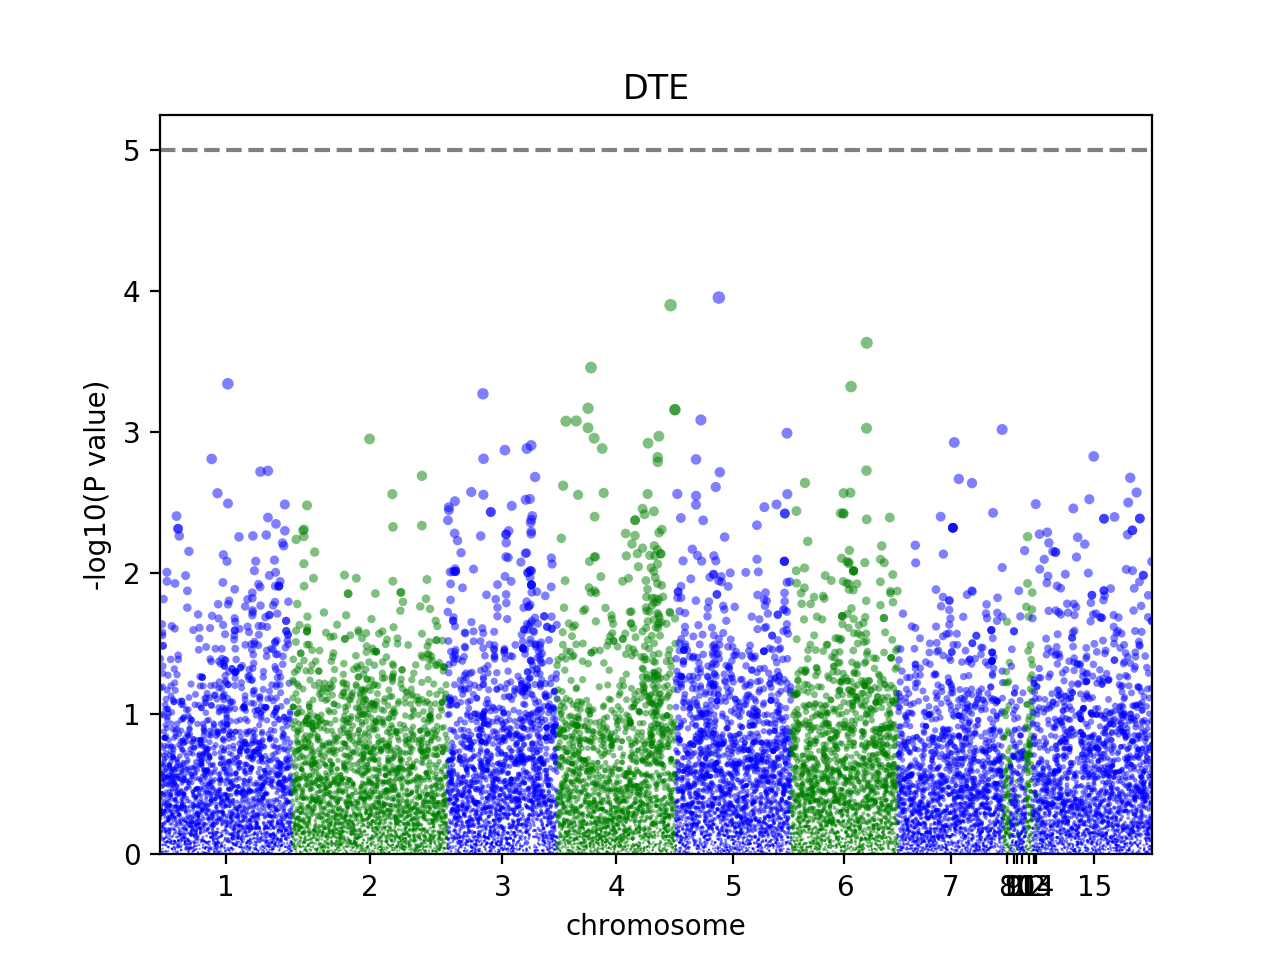
\includegraphics[scale=0.45]{FaST_LMM_DTE.png}
	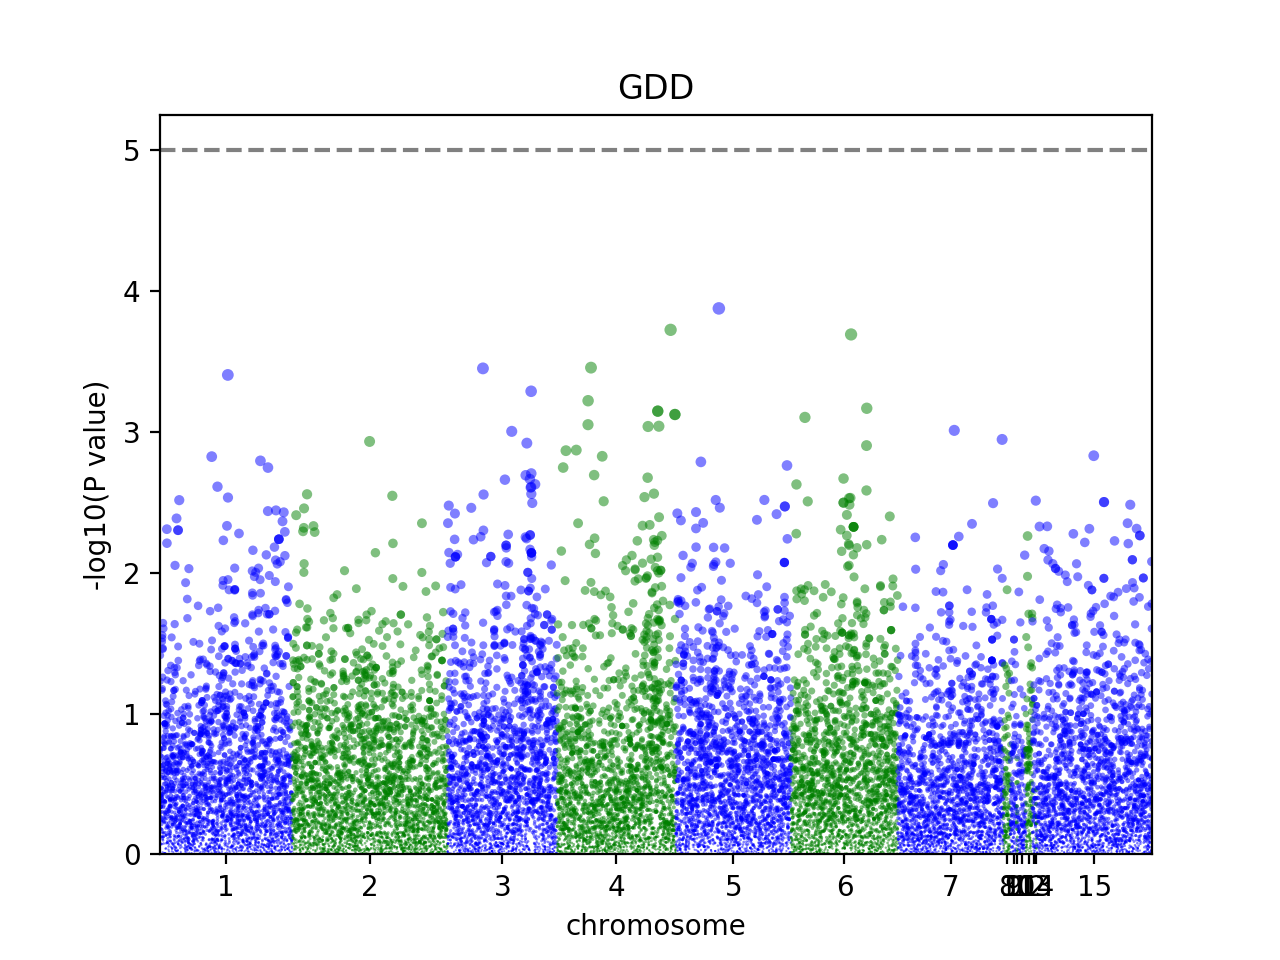
\includegraphics[scale=0.45]{FaST_LMM_GDD.png}
 	 \caption{Manhattan Plots of days to emergence and growing degree days GWAS results from Python FaST-LMM with environmental covariates}
 	 \label{fig:subfig1}
 \end{subfigure}
 
 \begin{subfigure}[normla]{\textwidth}
  \centering
	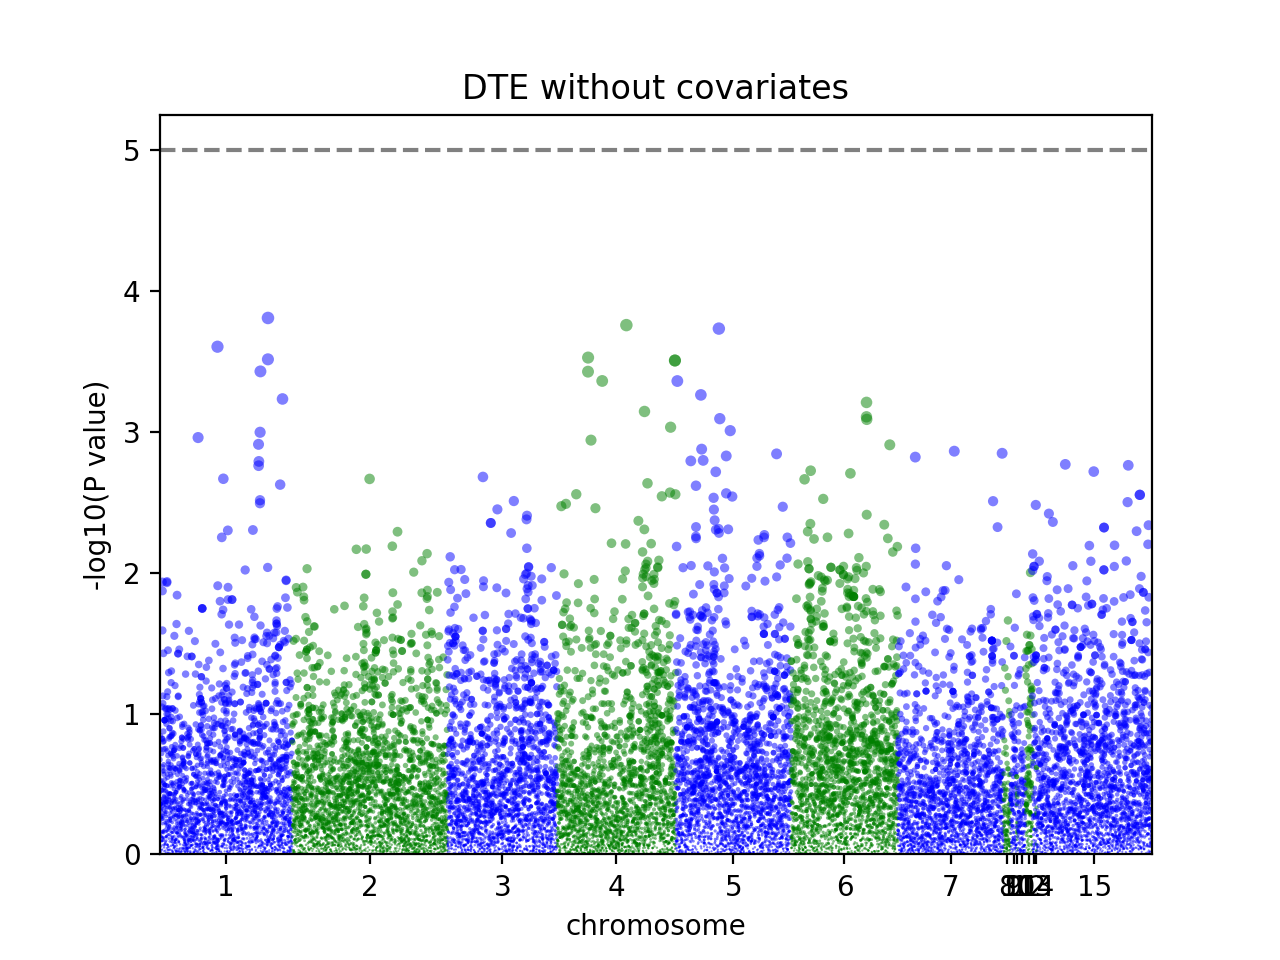
\includegraphics[scale=0.45]{FaST-LMM_DTE_ncov.png}
	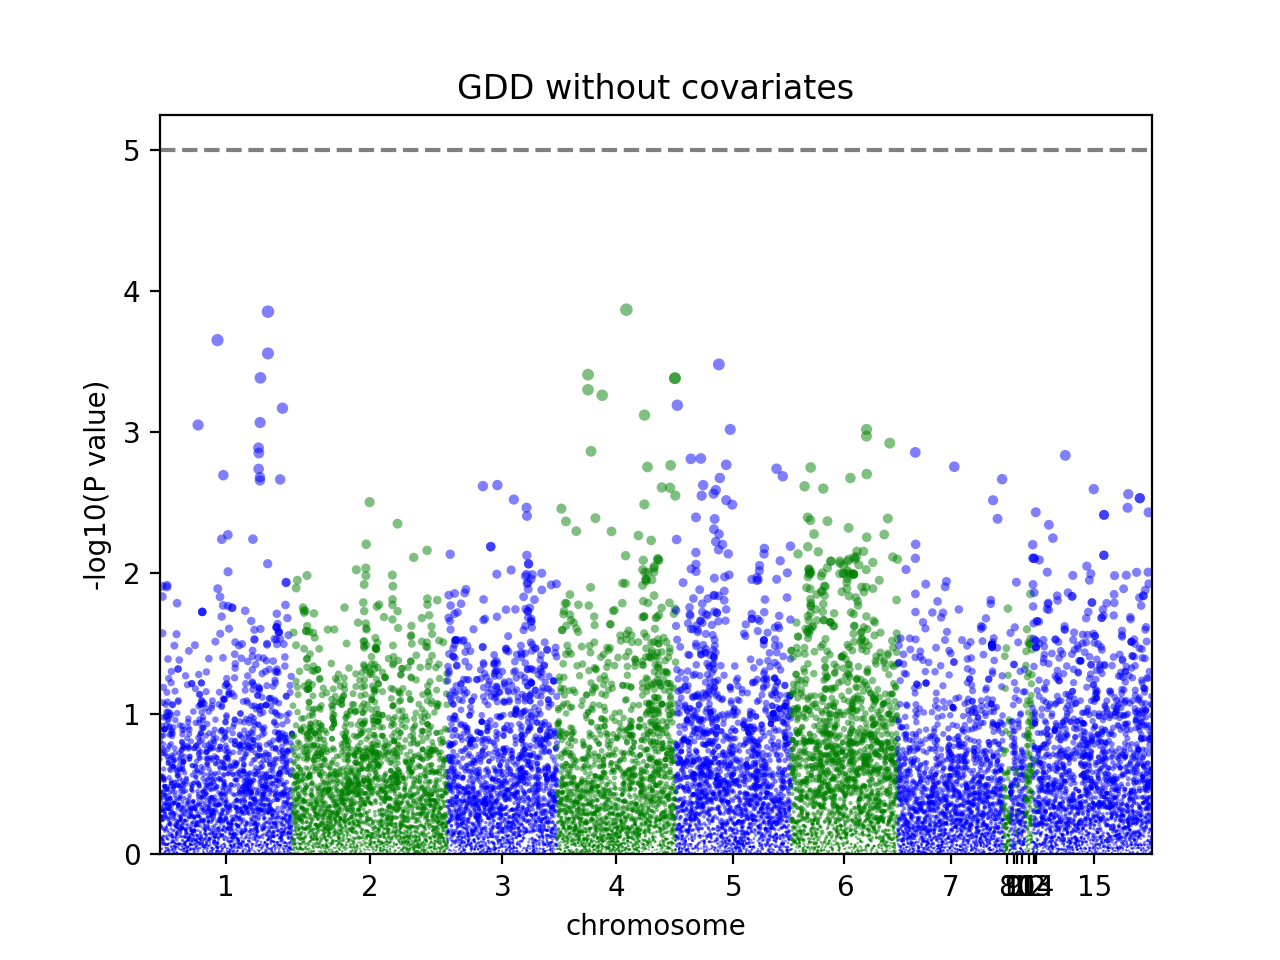
\includegraphics[scale=0.45]{FaST-LMM_GDD_ncov.png}
	\caption{Manhattan Plots of days to emergence and growing degrees days GWAS results from Python FaST-LMM without environmental covariates}
  \label{fig:subfig2}
 \end{subfigure}

\caption{Manhattan Plots of GWAS results from Python FaST-LMM}
\label{fig:fastlmm_res}
\end{figure}

%The quantile-quantile plot shown in Fig~\ref{fig2:qqplot} gives ... (needs to be completed)
\begin{figure}[!htb]
\centering
	\begin{subfigure}{\textwidth}
	\centering
		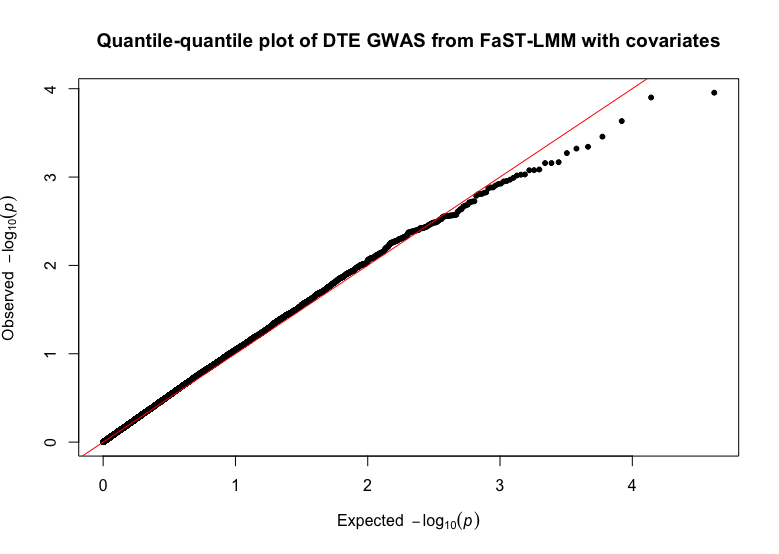
\includegraphics[scale=.25]{qqplot_fastlmm_dte_wcov.png}
		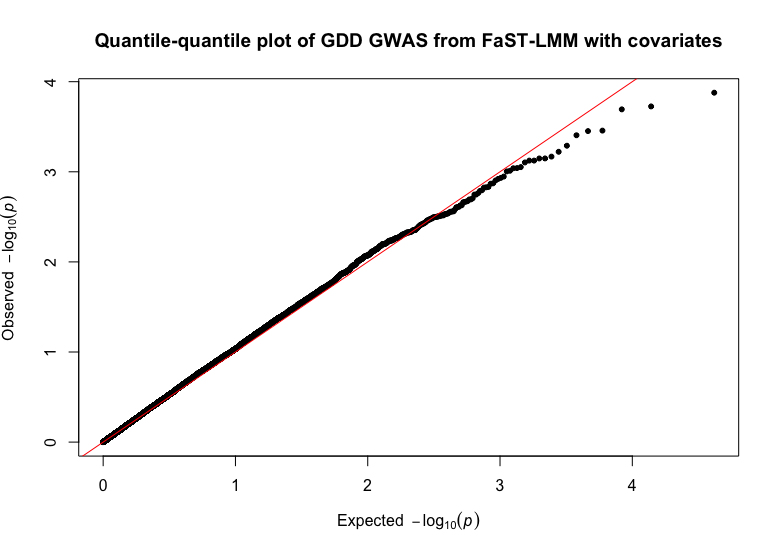
\includegraphics[scale=.25]{qqplot_fastlmm_gdd_wcov.png}
		\caption{Quantile-quantile plots of days to emergence and growing degree days GWAS from Python FaST-LMM with environmental covariates}
		\label{fig2:subfig1}
	\end{subfigure}
	
	\begin{subfigure}{\textwidth}
	\centering
		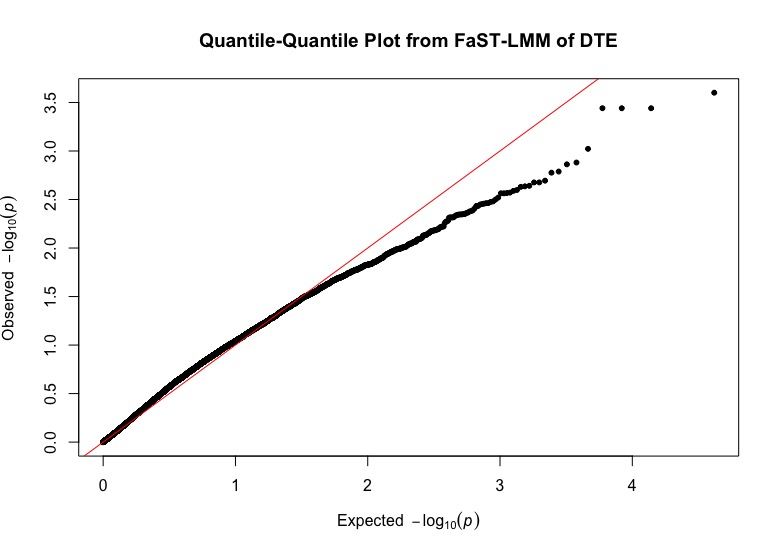
\includegraphics[scale=.25]{qqplot_fastlmm_dte.jpeg}
		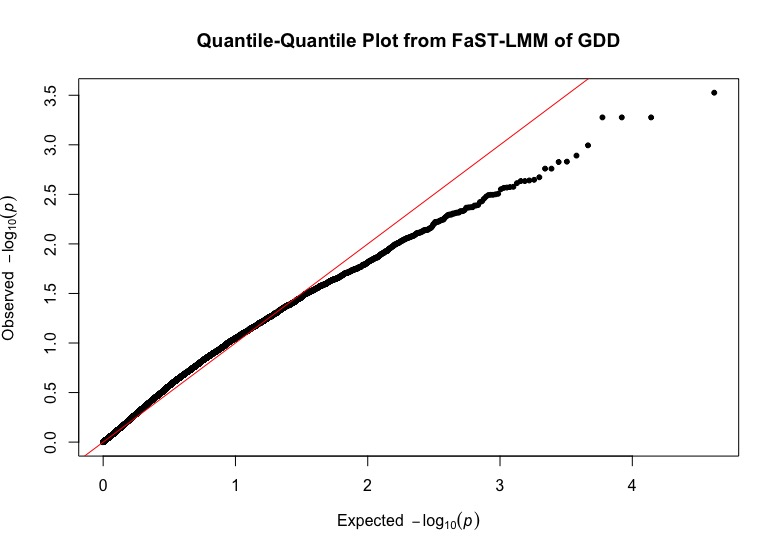
\includegraphics[scale=.25]{qqplot_fastlmm_gdd.jpeg}
		\caption{Quantile-quantile plots of days to emergence and growing degree days GWAS from Python FaST-LMM without environmental covariates}
		\label{fig2:subfig2}
	\end{subfigure}
\caption{Quantile-quantile plots of GWAS results from Python FaST-LMM}
\label{fig2:qqplot}
\end{figure}

According to Fig~\ref{fig:subfig1} and Fig~\ref{fig:subfig2}, it can be told that there are basically no significant SNPs in either of the two traits, which is opposite to that from PLINK. Additionally, the quantile-quantile plots shown in Fig~\ref{fig2:subfig1} and Fig~\ref{fig2:subfig2} indicate the results from Python FaST-LMM package follow the expected pattern and should be trusted. 

\end{document}